\documentclass[11pt]{article}

\usepackage{ctex}
\usepackage{bookmark}
\usepackage{listings}
\usepackage{epsfig}
\usepackage{lscape}
\usepackage{multirow}
\usepackage{longtable}
\usepackage{amsmath,amssymb,amsthm}
\usepackage{graphicx}
\usepackage{color}
\usepackage{placeins}
\usepackage{url}
\usepackage{cases}
\usepackage{hyperref}
\usepackage{setspace}
\usepackage{subfigure}
\usepackage{float}
\usepackage{framed}
\usepackage[c2]{optidef}
\usepackage{tikz}
\usepackage{caption}
\usepackage{algorithm}
\usepackage{algorithmic}
\usepackage{endnotes}
\usepackage{fontspec}


\usepackage{booktabs}

\oddsidemargin 0pt
\evensidemargin 0pt
\marginparwidth 10pt
\marginparsep 10pt
\topmargin -20pt
\textwidth 6.5in
\textheight 8.5in
\parindent = 20pt

\DeclareMathOperator*{\argmin}{argmin}
\DeclareMathOperator*{\minimax}{minimax}

\renewcommand{\algorithmicrequire}{ \textbf{function:}}
\renewcommand{\algorithmicreturn}{ \textbf{end function}}
\newcommand{\blue}[1]{\begin{color}{blue}#1\end{color}}
\newcommand{\magenta}[1]{\begin{color}{magenta}#1\end{color}}
\newcommand{\red}[1]{\begin{color}{red}#1\end{color}}
\newcommand{\green}[1]{\begin{color}{green}#1\end{color}}

\newtheorem{theorem}{Theorem}
\newtheorem{proposition}{Proposition}
\newtheorem{lemma}{Lemma}
\newtheorem{corollary}{Corollary}
\newtheorem{remark}{Remark}
\newtheorem{assumption}{Assumption}
\newtheorem{definition}{Definition}
%\newenvironment{proof}{{\noindent\it Proof}\quad}{\hfill $\square$\par}

%\usepackage{sidecap}


\definecolor{codegreen}{rgb}{0,0.6,0}
\definecolor{codegray}{rgb}{0.5,0.5,0.5}
\definecolor{codemauve}{rgb}{0.58,0,0.82}

\lstset{ %
	language=python,                % choose the language of the code
	basicstyle=\footnotesize\ttfamily,       % the size of the fonts that are used for the code
	numbers=left,                   % where to put the line-numbers
	numberstyle=\tiny\color{codegray},      % the size of the fonts that are used for the line-numbers
	stepnumber=1,                   % the step between two line-numbers. If it is 1 each line will be numbered
	numbersep=5pt,                  % how far the line-numbers are from the code
	backgroundcolor=\color{white},  % choose the background color. You must add \usepackage{color}
	showspaces=false,               % show spaces adding particular underscores
	showstringspaces=false,         % underline spaces within strings
	showtabs=false,                 % show tabs within strings adding particular underscores
	frame=single,                   % adds a frame around the code
	tabsize=4,                      % sets default tabsize to 4 spaces  
	captionpos=b,                   % sets the caption-position to bottom
	breaklines=true,                % sets automatic line breaking
	breakatwhitespace=false,        % sets if automatic breaks should only happen at whitespace
	escapeinside={\%*}{*)},
	commentstyle=\color{codegreen},
	keywordstyle=\bfseries\color{magenta},
	stringstyle=\color{red},
	identifierstyle=\color{codemauve},
	keepspaces=true
}


\begin{document}

\title{\bf Lab 1 实验报告}

\author{}
\date{\today}
\maketitle


\section{问题描述}

在上一个实验中,我们通过动态规划打表的方式完成了 LCS 的长度计算和结果输出,打表顺序是很自然的从左到右、从上到下,
但这种顺序构建的循环很显然是有数据依赖性的,根据状态转移方程,每一个 $ f(i, j+1) $ 都依赖于 $ f(i, j) $ 的结
果,因此我们在得到 $ f(i, j) $ 之前无法提前开始计算之后的格子,换言之这种朴素的算法并不具有并行性。

于是在这次实验中,我们将根据以下状态转移方程,设计新的打表顺序打破现有数据依赖性,以得到可以并行的程序。

$$
	f(i, j)= \begin{cases}
		0,                           & i<1 \text { or } j<1 \\
		f(i-1, j-1)+1,               & A[i]=B[j]            \\
		\max (f(i, j-1), f(i-1, j)), & A[i] \neq B[j]
	\end{cases}
$$


\section{算法设计}

如下图所示,注意到每一个格子的值仅与其左、上、左上的格子有关,于是沿着反对角线的方向构造内层循环,每次内层循环计算
一条反对角线,图中橙色表示已计算的格子,绿色表示正在计算的格子,灰色表示还未访问的格子,很明显绿色格子是可以并行计算
的。外层循环沿对角线方向进行。

\begin{figure}[H]
	\centering
	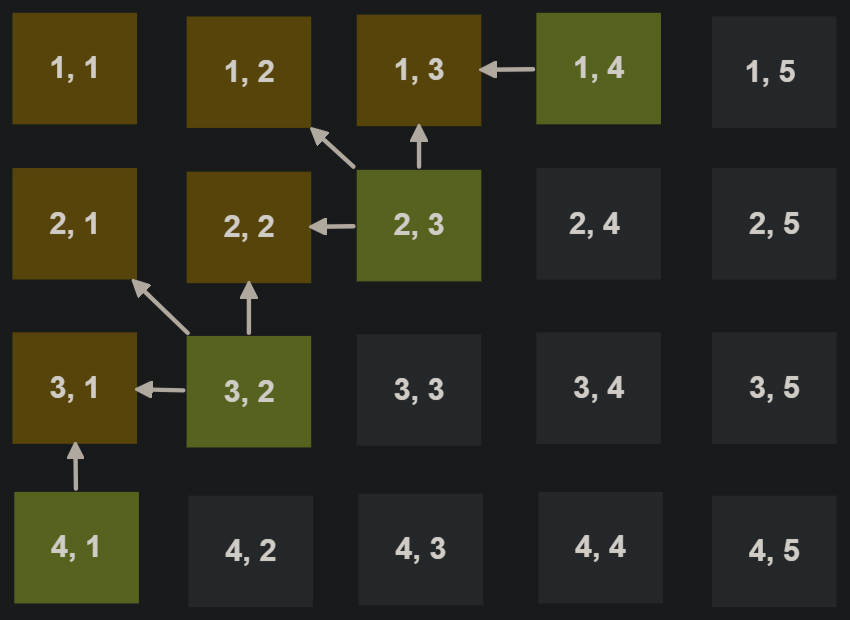
\includegraphics[width=0.5\textwidth]{./img/parallel-1.jpg}
	\caption{反对角线}
\end{figure}

于是将二维表旋转至反对角线水平方向,假设原索引 $ (i, j) $ 分别代表行序与列序,则新构建的双层循环变量 $ (s, t) $
满足 $ s=i+j $ 和 $ t=j-i $关系,具体实现只需再加一个偏移即可,再根据边界条件的区别分为三类,如图所示划分。

\begin{figure}[H]
	\centering
	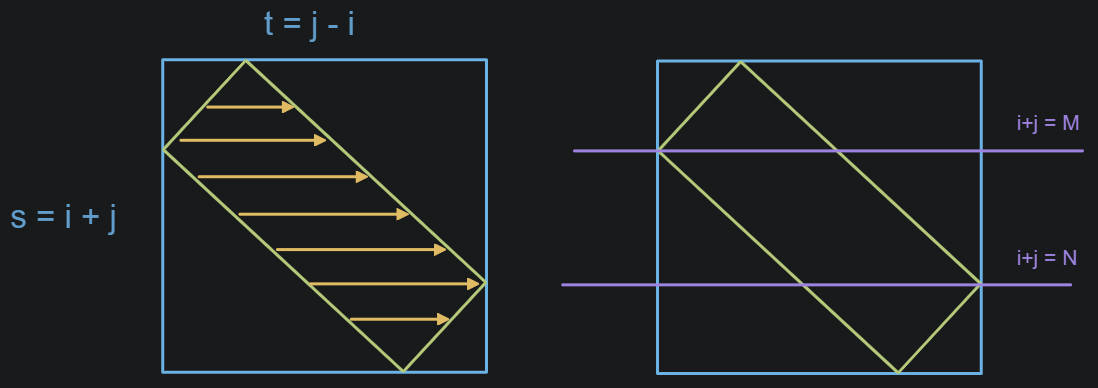
\includegraphics[width=0.7\textwidth]{./img/parallel-2.jpg}
	\caption{索引关系}
\end{figure}


\section{算法细节}

\begin{itemize}
	\item 受到 Lab0 参考答案的启发,设计使用一维数组存储动态规划表,空间复杂度减少至 $ O(M+N) $。
	\item 一开始将 for 循环分三类写,代码长而丑,后经助教指导合并为一个 for 循环,在外层循环计算内层循环边界条件即可,
	      美化代码,更具有可读性。
	\item 用三目运算符代替一些 if-else 分支,减少分支预测开销,且在 O3 优化中速度更快,实验表明有效。
	\item 在 cilk\_for 前编译指示颗粒度大小为 2048 (经粗略调参所得),减少并行产生的 block 数量,减少通讯开销。
\end{itemize}


\section{实验结果}

最早运行样例代码,在小阶数 (约 $ 10^4 $ 量级) 情况下出现反对角线并行速度慢于串行速度的异常情况。

\begin{figure}[H]
	\centering
	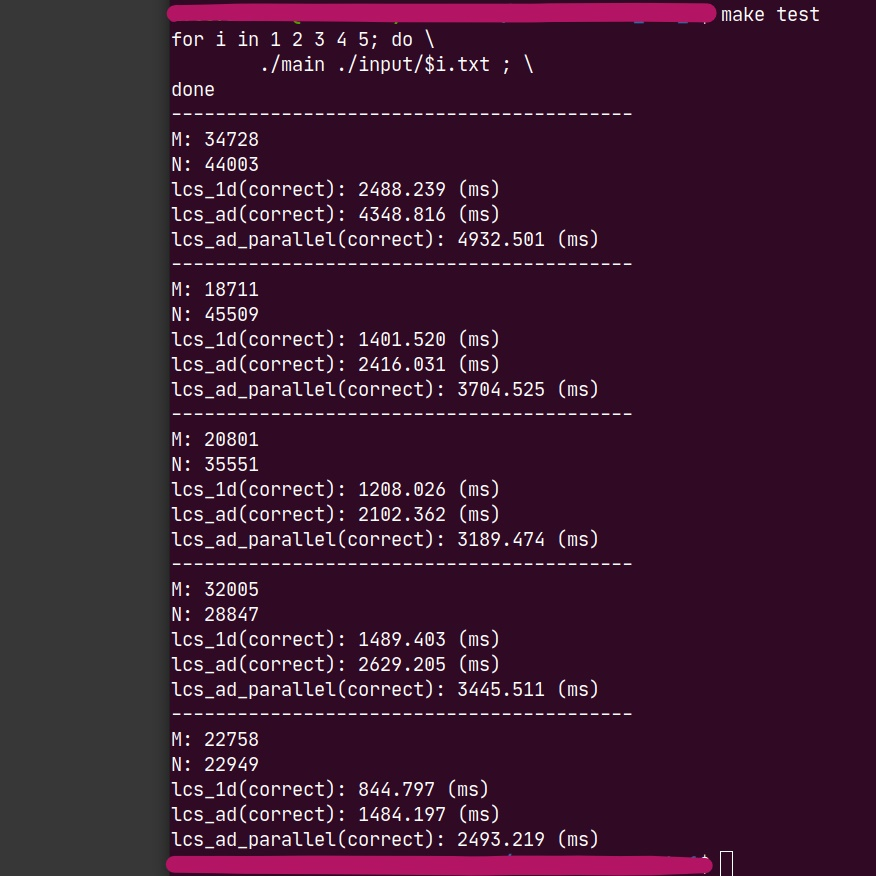
\includegraphics[width=0.45\textwidth]{./img/result-1.jpg}
	\caption{小阶数测试结果}
\end{figure}

后将阶数增大 (约 $ 10^5 $ 量级) ,反对角线并行速度远快于串行,并且超过朴素算法速度,证明了并行计算在大阶数情况下的
有效性。

\begin{figure}[H]
	\centering
	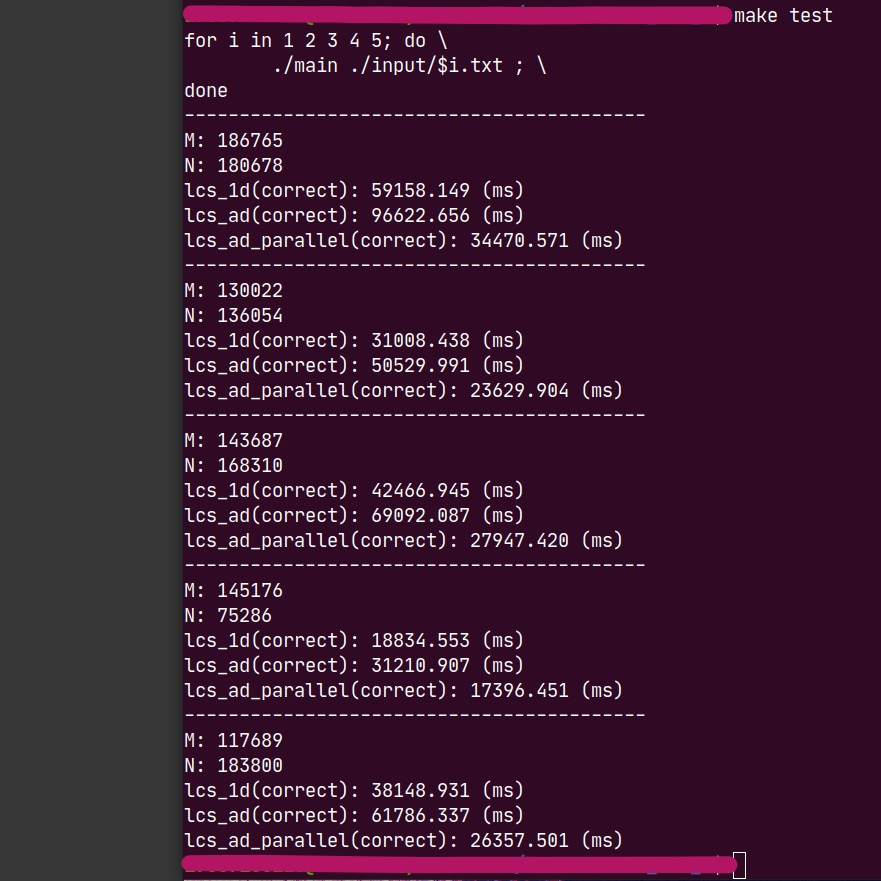
\includegraphics[width=0.45\textwidth]{./img/result-2.jpg}
	\caption{大阶数测试结果}
\end{figure}


\section{实验结果分析}

\begin{itemize}
	\item 小阶数情况下反对角线串行速度慢于朴素串行算法,可能是因为反对角线空间不连续导致的 cash miss 代价高于
	      O3 优化带来的加速,反对角线并行慢于反对角线串行的原因,可能是并行通讯开销代价高,总体不如 pipeline
	      优化速度。
	\item 大阶数情况下反对角线并行时间复杂度 $ O(n\log n) $,反对角线串行时间复杂度 $ O(n^2) $,在 $ n $
	      足够大时,会克服常数项趋向该加速比。
\end{itemize}


\end{document}


